
\chapter{Projekt i implementacja aplikacji internetowej w technologii Vue.js}
\section{Narzędzia i techonologie}
\subsection{Node.js}
Node.js~\cite{node} jest środowiskiem uruchomieniowym umożliwiającym używanie języka JavaScript poza przeglądarką. Środowisko to charakteryzuje asynchroniczność oraz sterowanie zdarzeniami. Asynchroniczność umożliwia wykonywanie wielu czynności w tym samym czasie bez względu na jednowątkowość wynikającą z ograniczenia języka JavaScript. Sterowanie zdarzeniami jest rozwiązaniem typowym dla interfejsów graficznych. Zapewnia ono elastyczność oraz możliwość tworzenia bardziej interaktywnych elementów GUI. Ponadto Node.js udostępnia menenadżera pakietów środowiska Node (NPM - Node Package Manager) dającego możliwość zarządzania zainstalowanymi funkcjonalnościami w prosty i przejrzysty sposób.
\subsection{Vue.js}
Vue.js~\cite{vue} to platforma programistyczna języka JavaScript służąca do budowania interfejsów użytkownika. W stosunku do dwóch najpopularniejszych alternatyw - platform programistycznych React oraz Angular - wyróżnia się prostotą, szybkością działania oraz niewielkim rozmiarem. Platforma programistyczna Vue.js została zaprojektowana tak, aby zapewnić jak największą elastyczność. Przy jej użyciu możliwe jest tworzenie nie tylko prostych komponentów, ale i aplikacji typu single-page-application oraz multi-page-application. 

Cechą charakterystyczną Vue.js jest wykorzystanie szablonów jako sposobu na powiązanie języka znaczników HTML z warstwą logiki JavaScript. Powiązanie to umożliwia wykorzystywanie w prosty sposób instrukcji warunkowych oraz pętli do wyświetlania zawartości aplikacji.   

\subsection{Vuex}
Vuex~\cite{vuex} to biblioteka oferująca scentralizowany magazyn danych dostępny dla wszystkich komponentów w aplikacji. Stan danych w magazynie Vuex jest zmieniany poprzez mutacje wykonywane w reakcji na działanie dyspozytora~(zob.~rysunek~\ref{rys:vuex}). Takie podejście sprawia, że dane z części backendowej aplikacji mogą zostać pobrane tylko raz, a później będą one dostępne bezpośrednio w części frontendowej za pośrednictwem magazynu.

\begin{figure}[t]
\centering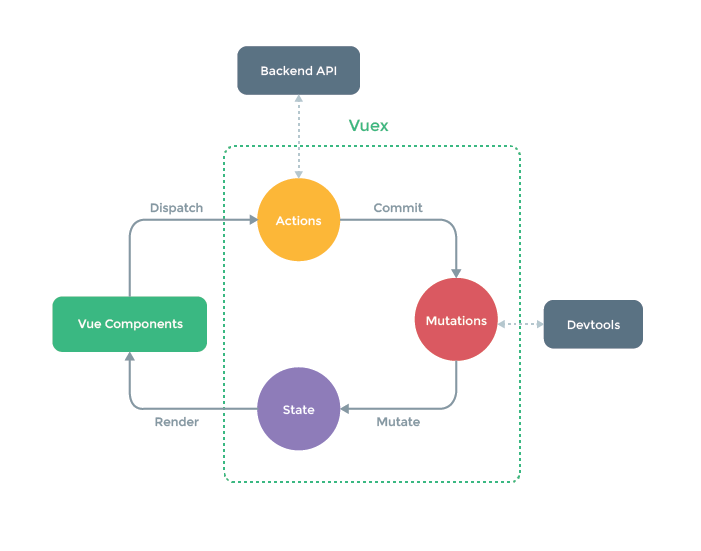
\includegraphics[width=\textwidth]{figures/vuex}
\caption{Schemat przepływu danych w Vuex~\cite{vuex2}}\label{rys:vuex}
\end{figure}

\subsection{Jest}
W projekcie wykorzystano testową platformę programistyczną Jest~\cite{jest} będącą częścią Vue Test Utils. Vue Test Utils to zestaw funkcjonalności upraszczających testowanie komponentów Vue.js. Zestaw ten zapewnia metody umożliwiające symulowanie działań użytkownika w aplikacji oraz przechwytywanie i porównywanie rezultatów tych interakcji z oczekiwanymi. Jest cechuje brak konieczności konfiguracji, izolacja testów oraz szybkość i bezpieczeństwo działania.
\subsection{Json Web Tokens}
Json Web Token~\cite{jwt} jest otwartym standardem przesyłania zabezpieczonych danych. Dane w formacie Json są podpisywane cyfrowo, co umożliwia weryfikację uprawnień. W aplikacjach internetowych JWT stosowane są głównie do autoryzacji użytkowników oraz zapewnienia bezpieczeństwa przesyłanie informacji pomiędzy frontendem a backendem. Niewielki rozmiar tokenu sprawia, iż możliwe jest przesyłanie go w treści zapytania HTTP lub nawet w jego nagłówku. Ta cecha sprawia również, że token może być przechowywany w pamięci przeglądarki, eliminując konieczność ponownego uwierzytelniania po rozpoczęciu nowej sesji.
\subsection{Postman}
Postman~\cite{postman} jest zestawem narzędzi do testowania API (Application Programming Interface). Zapewnia on możliwość wysyłania zapytań HTTP dowolnego typu oraz podgląd odpowiedzi i kodów błędów, jeśli takie wystąpiły. Główną zaletą Postmana jest możliwość tworzenia kolekcji zapytań, które ułatwiają organizację pracy podczas planowania połączeń pomiędzy częścią frontendową i backendową aplikacji. Dodatkowo narzędzie pozwala na współdzielenie kolekcji z zaproszonymi użytkownikami, co znacząco upraszcza proces testowania manualnego. Poza testowaniem manualnym Postman umożliwia tworzenie automatycznych testów przy pomocy języka JavaScript. Dzięki generatorowi losowych danych możliwa jest symulacja działań nawet kilku tysięcy różnych użytkowników w systemie.
\subsection{Visual Studio Code}
Visual Studio Code~\cite{vscode} jest edytorem kodu, którego głównymi zaletami jest wsparcie dla debugowania, inteligentnego uzupełniania kodu, refaktoryzacji oraz kontroli wersji. Dużą korzyścią płynącą z korzystania z programu Visual Studio Code jest dostęp do rozszerzeń, usprawniających pracę z kodem w dowolnym języku programowania. Rozszerzenia zapewniają również wsparcie dla platform programistycznych, w tym Vue.js, najbardziej istotnego dla tej części projektu. Mały rozmiar oraz wysoka wydajność znacznie przyśpieszają korzystanie z aplikacji i sprzyjają intensywnej iteracji rozwiązań.
\subsection{Axios}
Axios~\cite{axios} jest biblioteką języka JavaScript służącą do wykonywania zapytań HTTP z poziomu Node.js lub przeglądarki. W aplikacjach internetowych wykorzystywany jest do uzyskiwania danych z części backendowej aplikacji. Axios bazuje na obietnicach (promise), co pozwala na obsługiwanie akcji asynchronicznie. Biblioteka może być użyta poprzez zwykły Javascript lub platformę programistyczną taką jak Vue.js. W porównaniu z innymi bibliotekami służącymi do wykonywania zapytań HTTP Axios oferuje wsparcie dla starszych przeglądarek, możliwość ustawienia ograniczenia czasowego dla zapytań, ochronę przed CSRF (Cross-Site Request Forgery), a także automatyczną transformację danych JSON.
\subsection{Bootstrap}
Bootstrap~\cite{boot} jest platformą programistyczną CSS (Cascading Style Sheets) upraszczającą projektowanie interfejsu graficznego aplikacji internetowych. Bootstrap pomaga zapewnić responsywność stron, a więc poprawne ich wyświetlanie na urządzeniach mobilnych. Przed pojawieniem się tego rozwiązania często występowała konieczność przygotowywania oddzielnych stylów dla ekranów o rożnych rozdzielczościach. Dzięki zastosowaniu platformy programistycznej elementy strony internetowej zostają przeskalowane i przemieszczone tak, aby pomieścić się na ekranie niezależnie od jego wielkości i proporcji. Dodatkowo Bootstrap pozwala na zastosowanie zaawansowanych komponentów takich jak paski nawigacji, wskaźniki postępu czy miniatury. 
\section{Połączenie z backendem}
Połączenie z częścią backendową aplikacji jest realizowane przy pomocy biblioteki Axios. W tym celu wykorzystywane są dwa typy zapytań HTTP. Pierwszym z nich jest zapytanie typu GET. Przykładowym zastosowaniem tego zapytania jest odbieranie danych nauczycieli~(zob.~rysunek~\ref{rys:get}). Ze względu na fakt, że zapytanie typu GET nie posiada ciała wiadomości token uwierzytelniający JWT przesyłany jest w nagłówku. Dane zwrotne otrzymane z backendu zapisywane są w magazynie Vuex. Są tam również przechowywane informacje o powodzeniu operacji i komunikaty o błędzie, jeśli taki wystąpił.

\begin{figure}[h]
\centering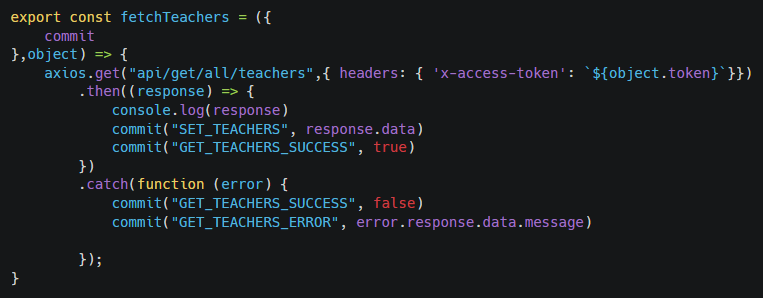
\includegraphics[width=\textwidth]{figures/get}
\caption{Funkcja wykonująca zapytanie typu GET}\label{rys:get}
\end{figure}

Drugim rodzajem zapytania HTTP wykorzystywanym do wymiany danych z backendem jest POST. W przeciwieństwie do komunikatu typu GET, komunikat typu POST posiada ciało wiadomości. Pozwala to na przesłanie tokenu uwierzytelniające w treści komunikatu. Przykładowym zastosowaniem zapytania tego typu jest przesyłanie danych nauczyciela~(zob.~rysunek~\ref{rys:post}). Poza tokenem uwierzytelniającym, w treści komunikatu przesyłane są informacje, które mają zostać zapisane w bazie danych. W odpowiedzi na komunikat zostaje przesłana informacja o powodzeniu operacji,a w przypadku niepowodzenia także komunikat o błędzie. Te dane są zapisywane w magazynie Vuex, co umożliwia ich wykorzystanie do wyświetlania komunikatów o błędzie użytkownikowi.
\begin{figure}[h]
\centering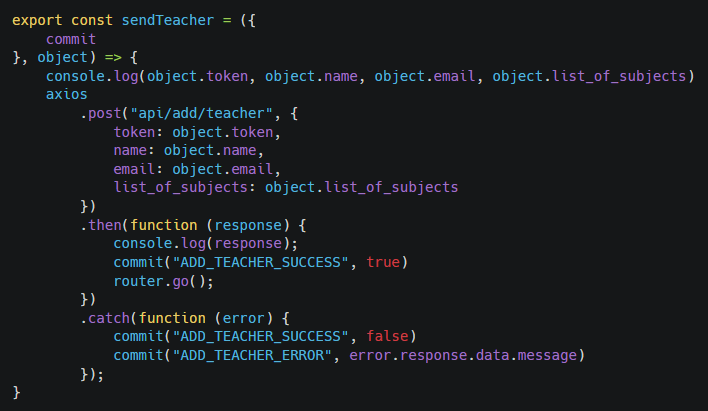
\includegraphics[width=\textwidth]{figures/post}
\caption{Funkcja wykonująca zapytanie typu POST}\label{rys:post}
\end{figure}




